\newcommand{\manycoreArchFigure}{
\begin{figure}[t]
    \centering
    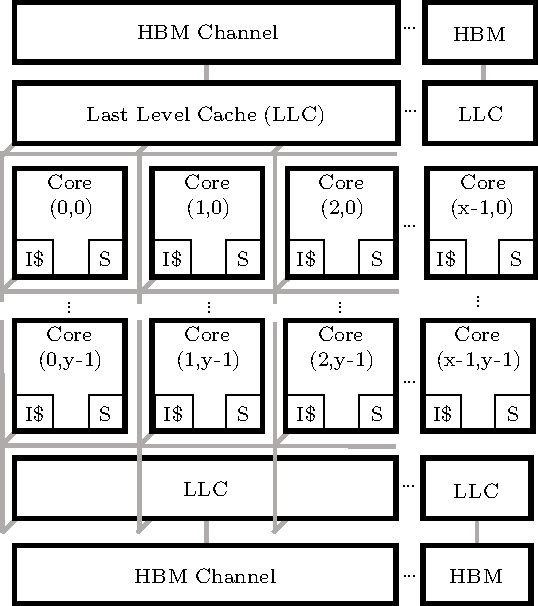
\includegraphics[scale=0.8]{graphit-figures/manycore-arch.pdf}
    \caption{Block diagram of the general manycore architecture targeted in
      this thesis. A 2D-Mesh Network-on-Chip connects general-purpose
      computation cores and Last Level Caches (LLC). Each LLC connects to a single
      independent High-Bandwidth Memory (HBM) channel.}
    \label{pap:generals:sec:architecture:fig:hbarch}
\end{figure}
}
\section{Manycore Architectures} \label{pap:generals:sec:architecture}
\manycoreArchFigure

Manycore architectures provide thread-level parallelism and flexibility with hundreds to thousands of general-purpose cores~\cite{ramey2011tilera, davidson2018celerity, gwennap2011adapteva, agathos2015parallela, taylor2004raw}.
Cores are arranged in two-dimensional arrays and interconnected with mesh-style networks for communication.
This network of cores is surrounded by multiple channels of memory to provide sufficient bandwidth and parallelism to sustain computation.
Cores within the architecture communicate explicitly through memory~\cite{davidson2018celerity} or message passing \cite{gwennap2011adapteva}, implicitly through coherence protocols~\cite{ramey2011tilera}, or both using inter-core result networks \cite{taylor2004raw}.
Communication allows cores to cooperate and solve large parallel tasks.
The quantity of cores and diverse communication patterns means that manycore architectures provide a flexible parallel computation fabric that can be tailored to fit application requirements or the structure of graph input data \cite{lumsdaine2007challenges}.

In this section, I describe a representative manycore architecture that we use to evaluate our code generator.
The cores are tiny, performance-optimized scalar cores that implement a RISC-V instruction set.
Each core has a software-managed scratchpad memory for low-latency storage and inter-thread communication.
Data cache lines do not move between cores, eliminating coherence overhead and false sharing.
The memory system is designed to expose memory parallelism and bandwidth to service memory requests from hundreds of concurrent threads.
This architecture is emblematic of Single Program Multiple Data (SPMD) parallel machines where collections of cores are loaded with the same program, but each core computes on different input data.

This section provides a overview of the target manycore
architecture depicted in
Figure~\ref{pap:generals:sec:architecture:fig:hbarch}. The
architecture is composed of efficient general-purpose processor cores,
Last Level Caches (LLCs), a 2D-Mesh Network on Chip, and High-Bandwidth
Memory (HBM) channels.
%% Fluff -M
%The system is designed for efficient
%computation of general-purpose scientific, graph, and machine-learning
%workloads that can exploit the unprecedented memory-level parallelism
%provided by the independent cores, caches, and HBM channels.



\subsection{Network-On-Chip}
Communication is provided by a 2D-Mesh Network-on-Chip (NoC) that
interconnects Last Level Caches and general-purpose cores. The
NoC supports point-to-point communication between endpoints using
shared memory. All addressable endpoints within the network are
assigned a unique global address range. This provides a PGAS-like
(Partitioned Global Address Space) memory model for execution.

\subsection{Memory System}
The manycore's memory system is designed to provide the high-bandwidth memory-level parallelism required by manycore
architectures. The memory system has four hierarchy levels:
High-Bandwidth Memory (HBM), Last Level Cache (LLC), core-remote
scratchpad (S), and core-local scratchpad (S). Each level is designed
to exploit memory parallelism and exposes a trade-off between latency,
capacity, as shown in
Figure~\ref{pap:generals:sec:architecture:fig:hbarch}.

Manycore architectures require many high-bandwidth and independent
memory channels to supply data for computation, so we use
second-generation High Bandwidth Memory (HBM, or HBM2). HBM provides
two sources of memory-level parallelism: First, HBM provides
channel-level parallelism with 8 independent physical channel
interfaces per chiplet. Each channel has a maximum data transfer rate of 32
GB/s. Second, HBM provides bank-level parallelism through pipelining
commands. Commands for opening/closing banks and reading data are
overlapped to hide the latency of long-running commands. Compared to
traditional SDRAM/DIMM-based devices, HBM provides more bandwidth
per-package and parallelism and is ideal for manycore
architectures, but performance depends on exploiting channel-level and
bank-level parallelism.

The banked Last Level Caches (LLC) shown in 
Figure~\ref{pap:generals:sec:architecture:fig:hbarch} are designed
to exploit bank-level parallelism within a channel. The LLCs are located at the top and bottom of the network to reduce memory access latency.
Each bank of the LLCs is connected
to a column and is mapped to a unique address range in the NoC, and
each port maps to an exclusive set of HBM banks within the LLC's
channel to avoid concurrency and conflicts. Linear traversals through
the memory space of a LLC expose bank-level parallelism to software.

% citation: https://user.eng.umd.edu/~blj/papers/memsys2018-dramsim.pdf
%Previous work has shown that for memory intensive workloads high memory bandwidth is often not enough to achieve good performance - it is also important that the memory system expose sufficient  memory level parallelism that software can exploit \cite{li2018ppmodernhighspeeddram}. 
%We use second-generation High Bandwidth Memory (HBM2) as our system's main memory. 
%HBM is a family of SDRAM technology that has recently gained prominence in parallel architectures such as GPGPUs and Google's TPU\todo{cite}. 
%HBM2 exposes two sources of memory-level parallelism. 
%First, HBM2's interface is composed of 8, independent memory channels each with wide interfaces. 
% An HBM2 channel can support up to 30 gigabytes per second of memory bandwidth. 
%Channels can receive memory requests and transfer data in parallel.
%The second way in which HBM provides MLP is in the number of DRAM banks.
%Within a bank only one memory page can be read at a time.
%Page conflicts arise when accessing data from two different pages located in the same bank. 
%When this occurs the currently opened page needs to closed, and the new page needs to be opened.
%Crucially, the operations for opening and closing pages in different banks can be overlapped. 
%Banks are thus another important source of parallelism in DRAM. 
%More banks means more open pages at a time, which reduces page conflicts when accessing DRAM and provides more opportunities to hide paging latency.
% An HBM2 chip has 16 DRAM banks per channel or 128 banks in total for the full 8 channel system.

%Our Last-Level Caches (LLC) are non-blocking with 128 byte blocks which is similar to the LLCs found in GPUs.
%We use one LLC for each HBM channel and are shown in Figure \ref{pap:generals:sec:architecture:fig:hbarch} at the top and bottom of the NoC.

%We design our cache system to exploit the MLP provided by HBM.
%The Last-Level Cache (LLC) is implemented using an array of power and area optimized blocking subcaches. 
%These subcaches operate independently and can handle  misses in parallel. 
%Each subcache services a physical address region that maps to a unique HBM bank. 
%An important consequence of this address mapping is that page conflicts can only occur from memory requests originating from the same blocking subcache.
%This maintains the memory system's ability to exploit bank level parallelism.
%It follows from our one-to-one assignment of subcaches to DRAM banks that each HBM channel handles memory requests from 16 blocking subcaches.
%The last-level cache uses 128 byte blocks, a configuration that we have found to be optimal for maximizing DRAM bandwidth and is\todo{cite} similar to what is found in GPGPU  architectures.
%The subcaches connect to the on-chip network at the top and bottom of each column in the mesh and sit between the compute cores and main system memory as shown in Figure \ref{pap:generals:sec:architecture:fig:hbarch}.


\subsection{Computational Cores}
The computational cores in
the manycore are
throughput-optimized, general purpose processors that communicate  over the NoC.
Each core is a modified Harvard architecture with an
instruction cache (I\$), and a small program-controlled data scratchpad
(S). Local scratchpad, remote scratchpads of other tiles, and main
memory are mapped to contiguous segments in the memory
space of each core. This allows nearby cores to communicate
using shared memory with extremely low overhead. 

Each core can issue a series of non-blocking, pipelined loads and stores to the NoC until a register hazard occurs. Multiple loads in flight exploit
instruction-based memory parallelism and hide the access latency of a
single access traversing the network (Table,
Figure~\ref{pap:generals:sec:architecture:fig:hbarch}). Operations
to sequential ports exploit bank-level memory parallelism, and
operations to unique caches exploit channel-level memory
parallelism. 
%The challenge for manycore architectures, and a major contribution of this paper, is to generate code that exploits the right types of parallelism to maximize performance for an application.
Manycore architectures with HBM are challenging to generate code for because of the interplay between bank and channel-level memory parallelism required to maximize performance for an application.

%Each core can issue many pipe-lined memory commands to the 
%NoC until the register file is exhausted, or a hazard occurs.
%Multiple loads in flight exploit instruction-level memory parallelism and
%hide the access latency of a single access traversing the network 
%(Table, Figure~\ref{pap:generals:sec:architecture:fig:hbarch}). 
%Loads to different memory banks exploit cache-level parallelism, and bank-level parallelism in the HBM. 
%Loads to different channels exploits channel-level memory parallelism. 
%The challenge for manycore architectures, and major contribution of this paper, is to generate code that 
%exploits the right types of parallelism to maximize performance for an application.

\subsection{Execution Model}
The manycore architecture operates under a Single Program Multiple
Data (SPMD) execution model where each core executes the same program
independently from all other cores. Multiple cores are aggregated into
rectangular \textit{groups} to perform computations that may require
cooperation. Cores in a group communicate through shared memory and
synchronize using dedicated barrier primitives. Groups can be executed
in parallel if resources are available, or sequentially if not. Ordering
between groups is not guaranteed. This programming abstraction can 
exploit the memory parallelism available in manycore architectures.

The manycore architecture described here is connected to a host	CPU, and
program execution is managed by a driver. Host programs	allocate
regions within the memory system and copy data from the host to the device,
launch parallel or sequential groups, and copy data back to the	host.
This process continues until all groups have launched and finished
execution. Once completed, the result can be copied back from the device
to host.